Первая составляющая формирователя - счётчик - во втором варианте ничем не отличается от первого. 5-разрядный выход счётчика подаётся на мультиплексор, который коммутирует один из своих 22 входов на выход. На дешифратор подаётся номер режима, данный узёл выставляет единицу на один из своих шести выходов в соответствии с режимом работы формирователя. Идея заключается в следующем: каждый из коммутируемых входов мультиплексора представляет собой один из 22-х импульсов в периодичной импульсной последовательности. Требуется установить в единицу только те импульсы, который должны присутствовать в данном режиме, остальные следует держать на нуле. Для достижения данной цели, выход из дешифратора, который соответствует определённому режиму, подаётся на те входы мультиплексора, которые соответствуют единичным импульсам в текущем режиме. Остальные импульсы, по природе работы дешифратора, будут нулями. Функциональная схема второго варианта представлена на рис. \ref{fig:secondnode}.
\begin{figure}
  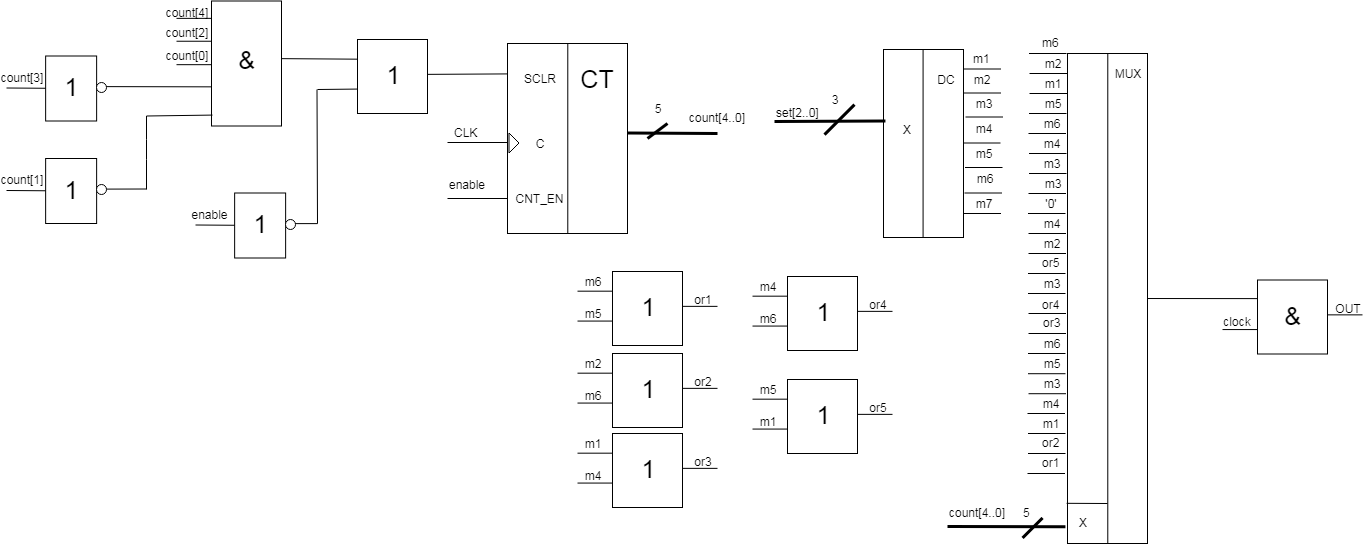
\includegraphics[scale=0.35]{./second-node.png}
  \caption{Функциональная схема многорежимного формирователя импульсной последовательности. Вариант 2.}
  \label{fig:secondnode}
\end{figure}